\chapter{Bottom-up block characterization and modeling}
\section{Characterizations}
\label{apx:block-cz}

\begin{figure}[!h]
  \centering
  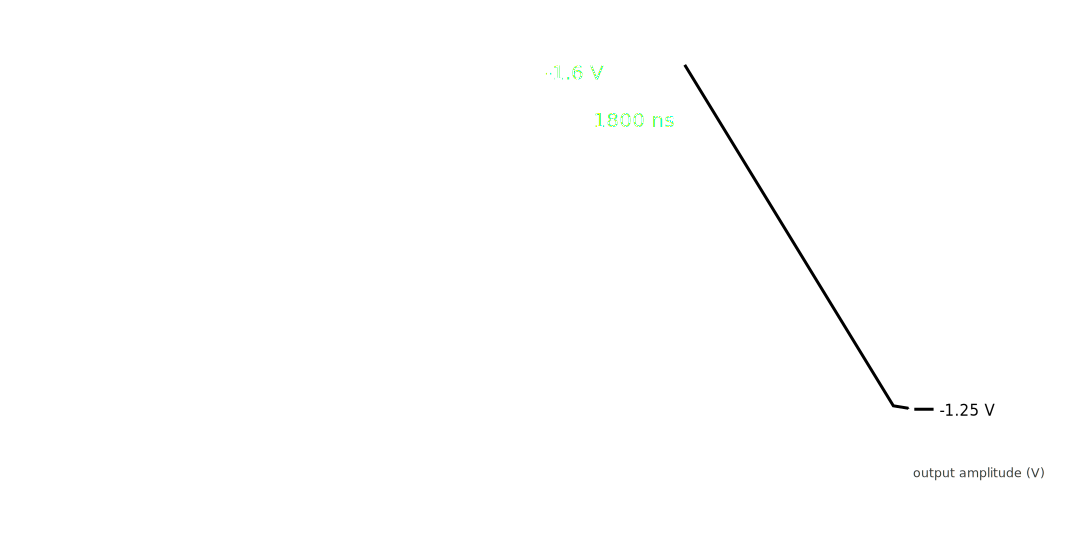
\includegraphics[width=\textwidth]{src/4/figures/bandgap_cz_v2_amp.pdf}
  \caption{Bandgap V\textsubscript{clamp9} amplitude matrix}
  \label{fig:bg_amp}
\end{figure}

\begin{figure}[!h]
  \centering
  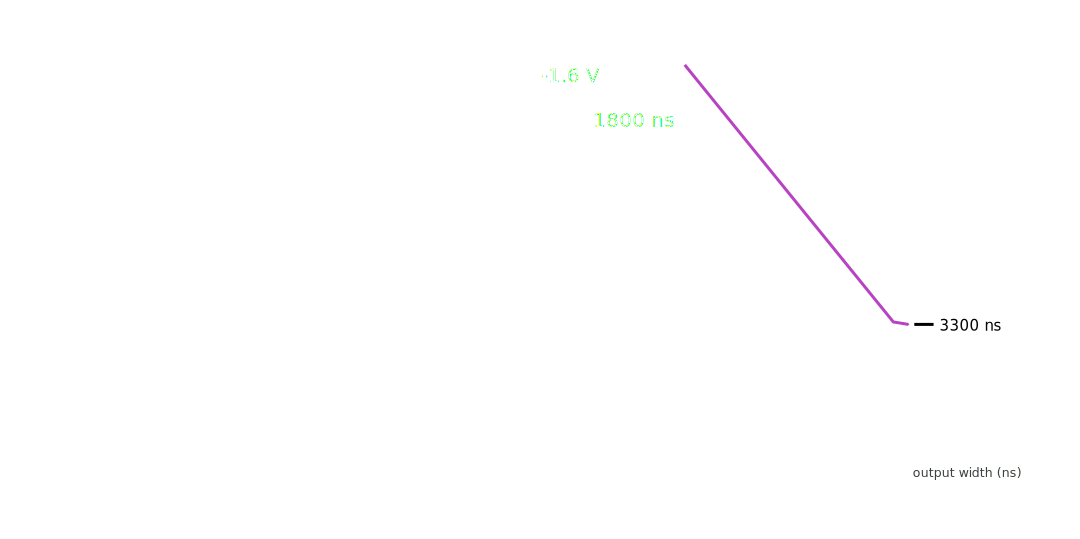
\includegraphics[width=\textwidth]{src/4/figures/bandgap_cz_v2_width.pdf}
  \caption{Bandgap V\textsubscript{clamp9} width matrix}
  \label{fig:bg_width}
\end{figure}

\begin{figure}[!h]
  \centering
  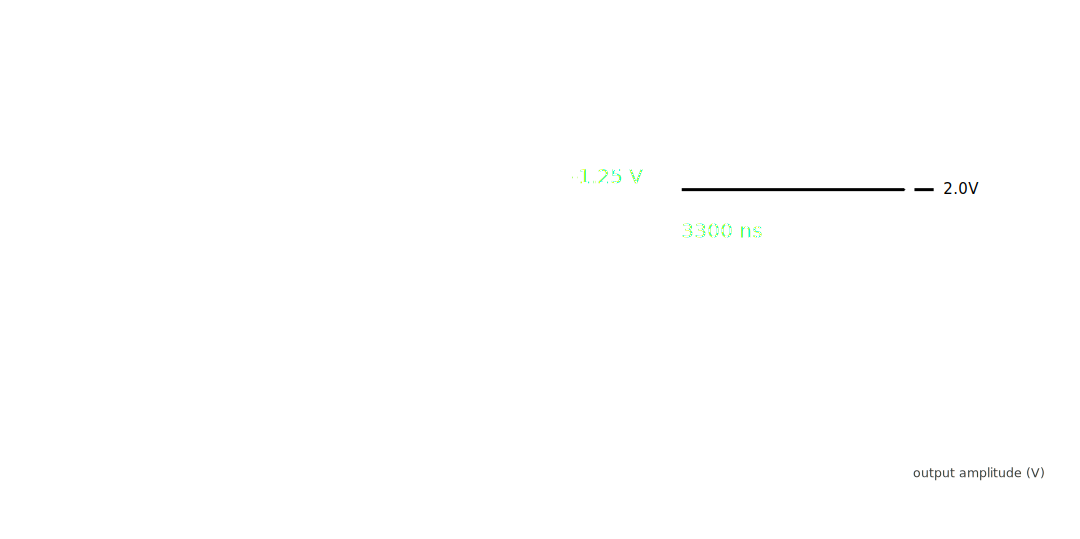
\includegraphics[width=\textwidth]{src/4/figures/regulator_cz_v2_amp.pdf}
  \caption{Regulator V\textsubscript{clamp9} amplitude matrix}
  \label{fig:regu_amp}
\end{figure}

\begin{figure}[!h]
  \centering
  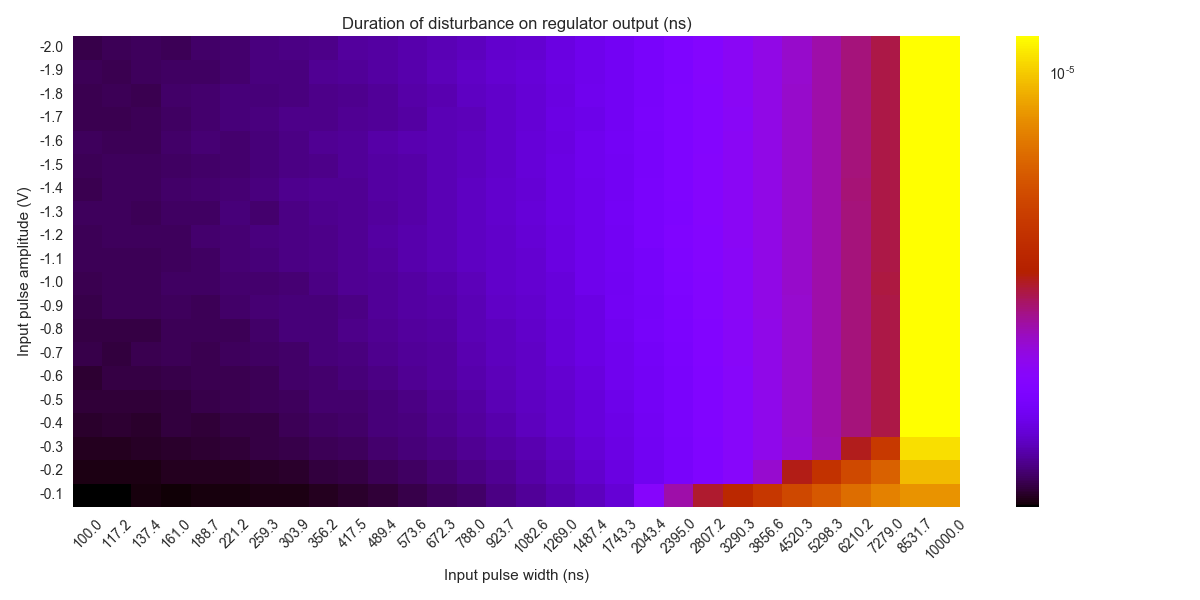
\includegraphics[width=\textwidth]{src/4/figures/regulator_cz_v2_width.pdf}
  \caption{Regulator V\textsubscript{clamp9} width matrix}
  \label{fig:regu_width}
\end{figure}

\section{Improved model chain versus reference}
\label{apx:block-model-comparison}

\begin{figure}[!h]
  \centering
  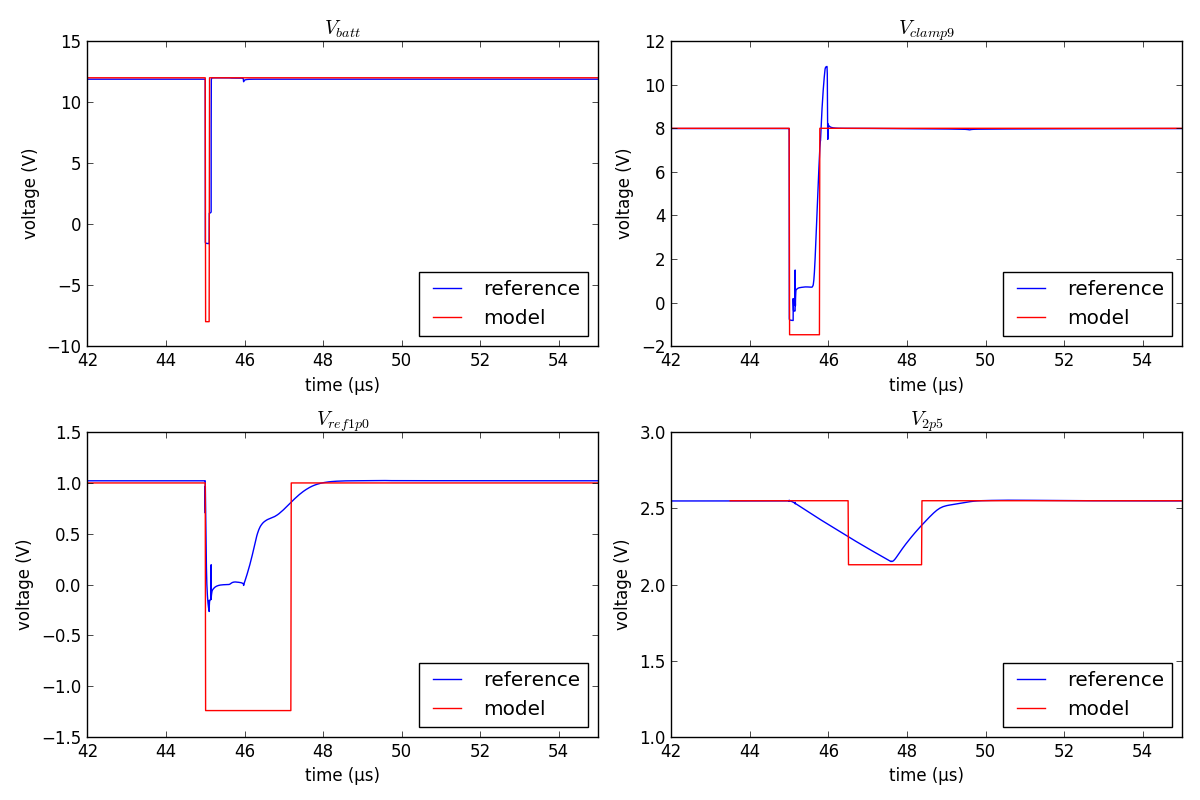
\includegraphics[width=\textwidth]{src/4/figures/total_simulation_20V_100n_V2.png}
  \caption{Reference versus model chain waveforms for a \SI{-20}{\volt} \SI{100}{\nano\second} stimulus}
  \label{fig:reference_simu_v2_20V_100n}
\end{figure}


\begin{figure}[!h]
  \centering
  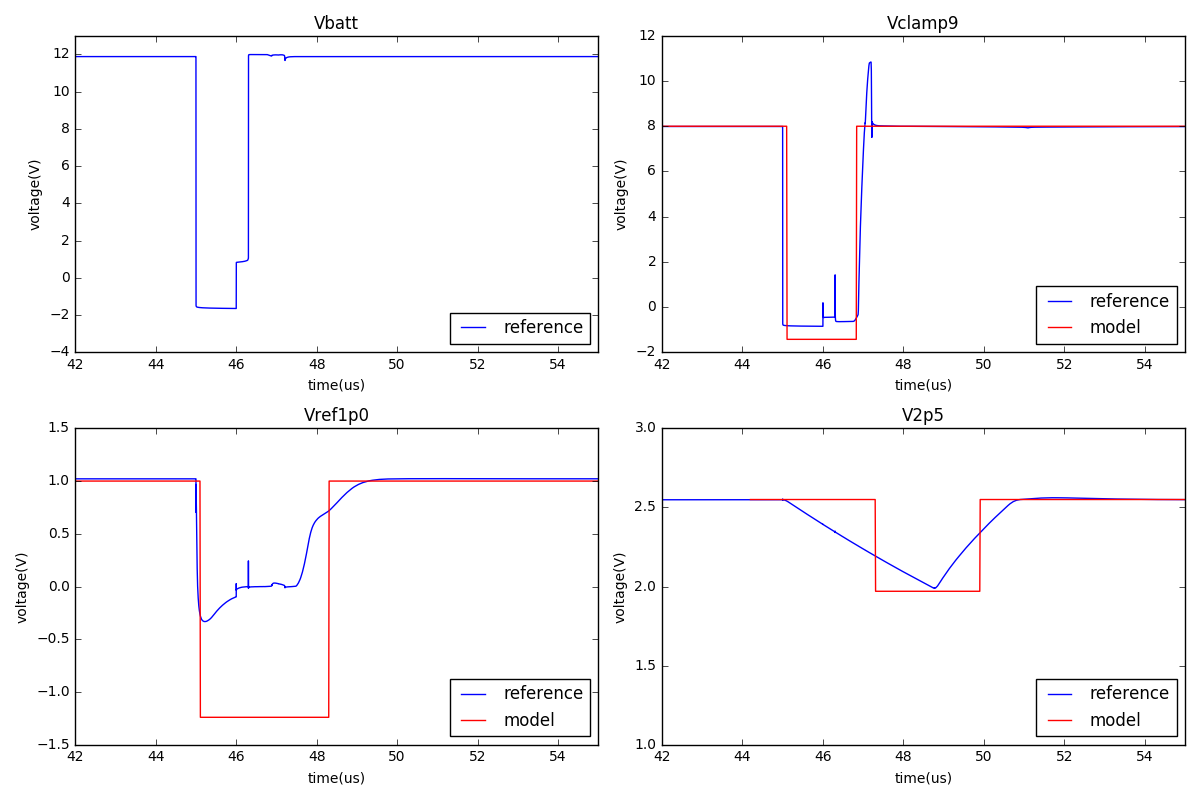
\includegraphics[width=\textwidth]{src/4/figures/total_simulation_20V_1u_V2.png}
  \caption{Reference versus model chain waveforms for a \SI{-20}{\volt} \SI{1}{\micro\second} stimulus}
  \label{fig:reference_simu_v2_20V_100n}
\end{figure}
